\documentclass{standalone}%
\usepackage[T1]{fontenc}%
\usepackage[utf8]{inputenc}%
\usepackage{lmodern}%
\usepackage{textcomp}%
\usepackage{lastpage}%
\usepackage{tikz}%
%
%
%
\begin{document}%
\normalsize%
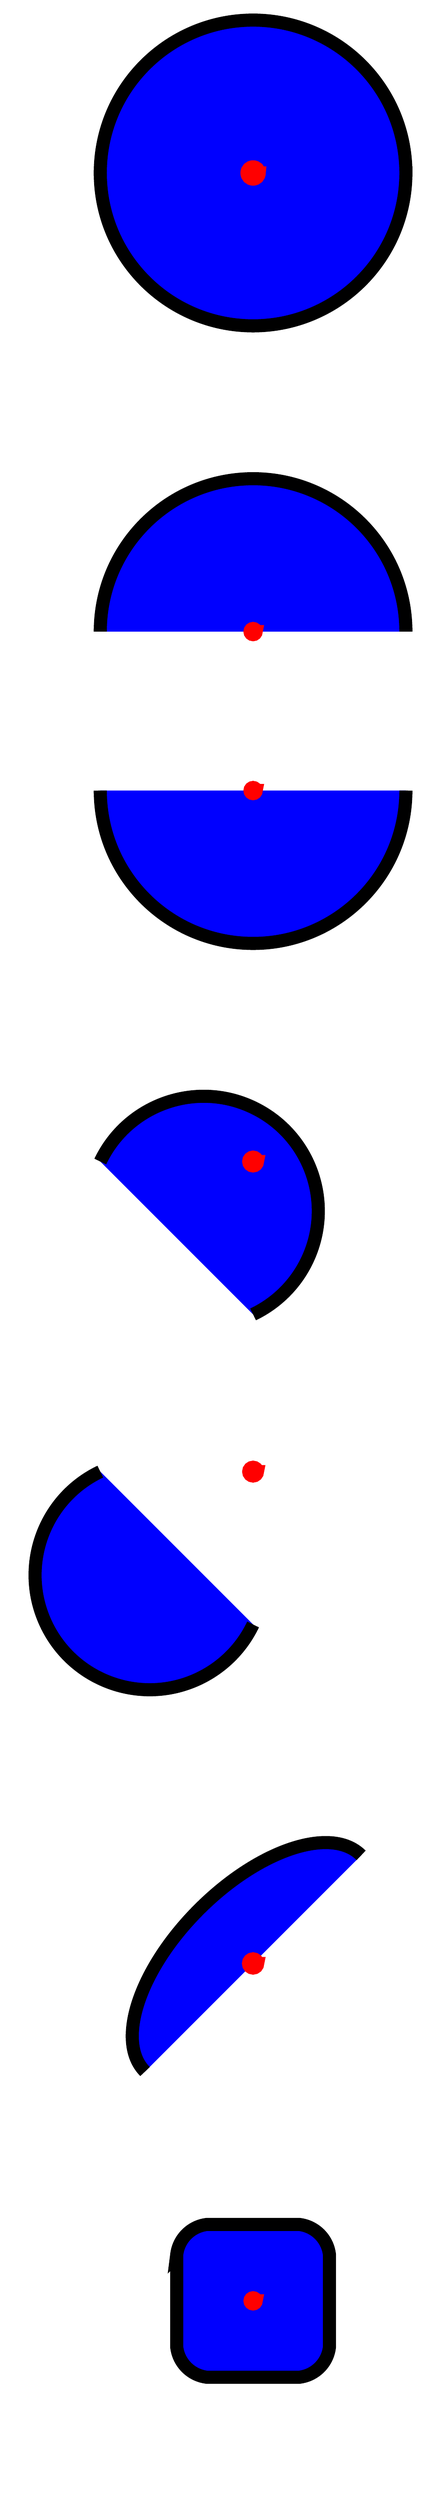
\begin{tikzpicture}%
\begin{scope}[cm={1.0, 0.0, 0.0, -1.0, (0.0, 0.0)}]%
\begin{scope}[cm={4.309091753604878, 0.0, 0.0, 4.309091753604878, (0.0, 0.0)}]%
\begin{scope}[cm={1.0, 0.0, 0.0, 1.0, (0.0, 0.0)}]%
\path[draw,fill={rgb,1:red,0.0; green,0.0; blue,1.0},line width=10.5pt] (1.0,0.0) {[rotate=0.0] arc[start angle=0.0, end angle=359.99999, x radius=1.0, y radius =1.0]} -- cycle;%
\end{scope}%
\begin{scope}[cm={1.0, 0.0, 0.0, 1.0, (0.0, 0.0)}]%
\path[draw,fill={rgb,1:red,0.0; green,0.0; blue,1.0},draw={rgb,1:red,1.0; green,0.0; blue,0.0},line width=10.5pt] (0.04,0.0) {[rotate=0.0] arc[start angle=0.0, end angle=359.99999, x radius=0.04, y radius =0.04]} -- cycle;%
\end{scope}%
\begin{scope}[cm={1.0, 0.0, 0.0, 1.0, (0.0, 1.5)}]%
\path (0.0,-0.5) rectangle (0.0,0.5);%
\end{scope}%
\begin{scope}[cm={1.0, 0.0, 0.0, 1.0, (0.0, 3.0)}]%
\begin{scope}[cm={1.0, 0.0, 0.0, 1.0, (0.0, 0.0)}]%
\path[draw,fill={rgb,1:red,0.0; green,0.0; blue,1.0},line width=10.5pt] (-1.0,0.0) {[rotate=-90.0] arc[start angle=270.0, end angle=450.0, x radius=1.0, y radius =1.0]};%
\end{scope}%
\begin{scope}[cm={1.0, 0.0, 0.0, 1.0, (0.0, 0.0)}]%
\path[draw,fill={rgb,1:red,0.0; green,0.0; blue,1.0},draw={rgb,1:red,1.0; green,0.0; blue,0.0},line width=10.5pt] (0.02,0.0) {[rotate=0.0] arc[start angle=0.0, end angle=359.99999, x radius=0.02, y radius =0.02]} -- cycle;%
\end{scope}%
\end{scope}%
\begin{scope}[cm={1.0, 0.0, 0.0, 1.0, (0.0, 3.52)}]%
\path (0.0,-0.5) rectangle (0.0,0.5);%
\end{scope}%
\begin{scope}[cm={1.0, 0.0, 0.0, 1.0, (0.0, 4.039999999999999)}]%
\begin{scope}[cm={1.0, 0.0, 0.0, 1.0, (0.0, 0.0)}]%
\path[draw,fill={rgb,1:red,0.0; green,0.0; blue,1.0},line width=10.5pt] (-1.0,0.0) {[rotate=90.0] arc[start angle=90.0, end angle=-90.0, x radius=1.0, y radius =1.0]};%
\end{scope}%
\begin{scope}[cm={1.0, 0.0, 0.0, 1.0, (0.0, 0.0)}]%
\path[draw,fill={rgb,1:red,0.0; green,0.0; blue,1.0},draw={rgb,1:red,1.0; green,0.0; blue,0.0},line width=10.5pt] (0.02,0.0) {[rotate=0.0] arc[start angle=0.0, end angle=359.99999, x radius=0.02, y radius =0.02]} -- cycle;%
\end{scope}%
\end{scope}%
\begin{scope}[cm={1.0, 0.0, 0.0, 1.0, (0.0, 5.539999999999999)}]%
\path (0.0,-0.5) rectangle (0.0,0.5);%
\end{scope}%
\begin{scope}[cm={1.0, 0.0, 0.0, 1.0, (0.0, 6.466776695296636)}]%
\begin{scope}[cm={1.0, 0.0, 0.0, 1.0, (0.0, 0.0)}]%
\path[draw,fill={rgb,1:red,0.0; green,0.0; blue,1.0},line width=10.5pt] (-1.0,1.1102230246251565e-16) {[rotate=-44.999999999999986] arc[start angle=-109.4712206344907, end angle=109.47122063449068, x radius=0.7499999999999999, y radius =0.7499999999999999]};%
\end{scope}%
\begin{scope}[cm={1.0, 0.0, 0.0, 1.0, (0.0, 0.0)}]%
\path[draw,fill={rgb,1:red,0.0; green,0.0; blue,1.0},draw={rgb,1:red,1.0; green,0.0; blue,0.0},line width=10.5pt] (0.02853553390593273,0.0) {[rotate=0.0] arc[start angle=0.0, end angle=359.99999, x radius=0.02853553390593273, y radius =0.02853553390593273]} -- cycle;%
\end{scope}%
\end{scope}%
\begin{scope}[cm={1.0, 0.0, 0.0, 1.0, (0.0, 7.966776695296636)}]%
\path (0.0,-0.5) rectangle (0.0,0.5);%
\end{scope}%
\begin{scope}[cm={1.0, 0.0, 0.0, 1.0, (0.0, 8.495312229202568)}]%
\begin{scope}[cm={1.0, 0.0, 0.0, 1.0, (0.0, 0.0)}]%
\path[draw,fill={rgb,1:red,0.0; green,0.0; blue,1.0},line width=10.5pt] (-1.0,1.1102230246251565e-16) {[rotate=135.00000000000003] arc[start angle=-250.52877936550934, end angle=-469.4712206344907, x radius=0.7499999999999999, y radius =0.7499999999999999]};%
\end{scope}%
\begin{scope}[cm={1.0, 0.0, 0.0, 1.0, (0.0, 0.0)}]%
\path[draw,fill={rgb,1:red,0.0; green,0.0; blue,1.0},draw={rgb,1:red,1.0; green,0.0; blue,0.0},line width=10.5pt] (0.028535533905932733,0.0) {[rotate=0.0] arc[start angle=0.0, end angle=359.99999, x radius=0.028535533905932733, y radius =0.028535533905932733]} -- cycle;%
\end{scope}%
\end{scope}%
\begin{scope}[cm={1.0, 0.0, 0.0, 1.0, (0.0, 10.422088924499205)}]%
\path (0.0,-0.5) rectangle (0.0,0.5);%
\end{scope}%
\begin{scope}[cm={1.0, 0.0, 0.0, 1.0, (0.0, 11.7126583395413)}]%
\begin{scope}[cm={1.0, 0.0, 0.0, 1.0, (0.0, 0.0)}]%
\path[draw,fill={rgb,1:red,0.0; green,0.0; blue,1.0},line width=10.5pt] (-0.7071067811865476,0.7071067811865475) {[rotate=-135.0] arc[start angle=270.0, end angle=450.0, x radius=0.5, y radius =1.0]};%
\end{scope}%
\begin{scope}[cm={1.0, 0.0, 0.0, 1.0, (0.0, 0.0)}]%
\path[draw,fill={rgb,1:red,0.0; green,0.0; blue,1.0},draw={rgb,1:red,1.0; green,0.0; blue,0.0},line width=10.5pt] (0.029953523924572845,0.0) {[rotate=0.0] arc[start angle=0.0, end angle=359.99999, x radius=0.029953523924572845, y radius =0.029953523924572845]} -- cycle;%
\end{scope}%
\end{scope}%
\begin{scope}[cm={1.0, 0.0, 0.0, 1.0, (0.0, 12.919765120727847)}]%
\path (0.0,-0.5) rectangle (0.0,0.5);%
\end{scope}%
\begin{scope}[cm={1.0, 0.0, 0.0, 1.0, (0.0, 13.919765120727847)}]%
\begin{scope}[cm={1.0, 0.0, 0.0, 1.0, (-0.49999999999999994, -0.5)}]%
\path[draw,fill={rgb,1:red,0.0; green,0.0; blue,1.0},line width=10.5pt] (0.0,0.2) -- (0.0,0.8) {[rotate=135.00000000000003] arc[start angle=38.942441268981355, end angle=-38.94244126898138, x radius=0.22500000000000003, y radius =0.22500000000000003]} -- (0.8,1.0) {[rotate=45.00000000000001] arc[start angle=38.942441268981376, end angle=-38.94244126898139, x radius=0.22499999999999998, y radius =0.22499999999999998]} -- (1.0,0.2) {[rotate=-44.99999999999999] arc[start angle=38.94244126898137, end angle=-38.94244126898139, x radius=0.22500000000000003, y radius =0.22500000000000003]} -- (0.2,0.0) {[rotate=-135.0] arc[start angle=38.94244126898137, end angle=-38.94244126898138, x radius=0.2250000000000001, y radius =0.2250000000000001]} -- cycle;%
\end{scope}%
\begin{scope}[cm={1.0, 0.0, 0.0, 1.0, (0.0, 0.0)}]%
\path[draw,fill={rgb,1:red,0.0; green,0.0; blue,1.0},draw={rgb,1:red,1.0; green,0.0; blue,0.0},line width=10.5pt] (0.02,0.0) {[rotate=0.0] arc[start angle=0.0, end angle=359.99999, x radius=0.02, y radius =0.02]} -- cycle;%
\end{scope}%
\end{scope}%
\end{scope}%
\end{scope}%
\begin{scope}[cm={1.0, 0.0, 0.0, 1.0, (-0.965485467625077, -30.359174588947436)}]%
\path (-5.490031808910199,-34.883720930232556) rectangle (5.490031808910199,34.883720930232556);%
\end{scope}%
\end{tikzpicture}%
\end{document}